\documentclass[twocolumn]{aastex63}
\usepackage{natbib}
%\definecolor{orcidlogocol}{HTML}{A6CE39}
\bibliographystyle{aasjournal}

\begin{document}

\title{COLLISION RATES OF PLANETESIMALS NEAR MEAN-MOTION RESONANCES}

\author{Spencer C. Wallace}
\affiliation{Astronomy Department, University of Washington, Seattle, WA 98195}

\author{Aaron C. Boley}
\affiliation{Department of Physics and Astronomy, University of British Columbia, Vancouver BC, Canada}

\author{Thomas R. Quinn}
\affiliation{Astronomy Department, University of Washington, Seattle, WA 98195}

\begin{abstract}
A perturbing planet can leave a lasting imprint a debris disk near the locations of mean motion resonances (MMRs). Unfortunately, the planetesimal-sized objects that make up the majority of these disks are extremely difficult to directly observe. Dust created from collisions between planetesimals may be a much better way to constrain the structure of these disks. We use a direct N-body model to measure planetesimal collision rates in a dynamically cold debris disk composed of 150 km bodies. Even though the eccentricities are pumped at the nominal resonance locations, conservation of the Jacobi energy pushes planetesimals inward and enhances the collision rate adjacent to the resonances. In addition, we find that the collision rate is severely throttled near the 3:1 MMR and that a tightly wound spiral wave is launched from this location.
\end{abstract}

\section{Introduction} \label{sec:intro}

Recent observations of circumstellar disks by ALMA have revealed a rich variety of substructure in the millimeter wavelength contiunuum emission. Features such as gaps and asymmetries \citep{2015ApJ...808L...3A, 2016Sci...353.1519P, PhysRevLett.117.251101, 2016ApJ...820L..40A, 2016Natur.535..258C} in the emission provide diagnostics for the physical processes that drive the evolution of the disks. At these wavelengths, much of this light is produced by second-generation debris generated through collisional grinding of planetesimals \citep[see][]{2008ARA&A..46..339W}. 

In some cases, these gap features are argued to be an indicator for the presence of a giant planet, either embedded in the disk \citep{2015MNRAS.453L..73D} or orbiting externally. An giant perturber can influence the structure of the dust emission in a number of ways. A misaligned giant planet can produce nonaxisymmetric features such as warps \citep{2001A&A...370..447A}. Highly eccentric perturbers can produce even more complicated structures through secular perturbations \citep{2014MNRAS.443.2541P, 2015MNRAS.448.3679P}. Mean motion resonances (MMRs) have been shown to open gaps as well \citep{2015ApJ...798...83N, 2016ApJ...818..159T, 2018ApJ...857....3T}.

The dynamics governing the motion of bodies near MMRs is extremely nonlinear, as is determining what the collision rates between planetesimals should look like in these regions. For a collection of bodies massive enough to experience the effects of gravitational focusing, a large eccentricity dispersion tends to reduce the probability of collision, while enhancements in surface density tends to increase it. Due to conservation of the Jacobi energy, MMRs simultaneously enhance the local eccentricity dispersion and also enhance the surface density adjacent to the resonance \citep{2000Icar..143...45R, 2017ApJ...850..103B}.

Because the second generation dust production is driven by the planetesimal collision rate, it is crucial to understand how the dynamics that drive collisions works. In particular, it is not obvious how to link the readily observable thermal emission from dust in protoplanetary disks to the presence of a perturbing giant planet. Due to its nonlinearity, this problem is best studied with N-body simulations. Unfortunately, collision detection in an N-body simulation is extremely computationally expensive. So far, studies of planetesimal dynamics near MMRs have involved either collisionless test particles \citep{2017ApJ...850..103B, 2016ApJ...818..159T, 2018ApJ...857....3T} or severely limited integration times \citep{2000Icar..143...45R}.

To further elucidate this subject, we use the tree based N-body code {\sc ChaNGa} \citep{2008IEEEpds...ChaNGa, 2015AphCom..2..1} to follow the collisional evolution of a planetesimal disk under the gravitational influence of a Jupiter sized body. Because particle positions are sorted into a tree structure, neighbor finding and collision detection can be done quickly and efficiently. This considerably relaxes the constraints on resolution and integration time. With this toolset, we explore the collision rate structure of the planetesimal disk in the vicinity of mean motion resonances.

This work is organized in the following way. In section \ref{sec:dynamics} we provide an overview of the dynamics that drive the evolution of a planetesimal disk under the gravitational influence of an external perturber. In section \ref{sec:setup} we describe the N-body code we use and describe how we constructed the initial conditions for the two simulations that are run: one with a perturber on a circular orbit and one with an eccentric perturber. Section \ref{sec:results} goes on to explore the results of the two, with particular focus on the radial variation in the collision rates. In section \ref{sec:dust}, we use the positions of the collision events to construct a map of second generation dust emission, under the assumption that dust grains produced by collisions will immediately couple to the gas and circularize their orbits. Finally, we assess the observability of features in the dust emission due to mean motion resonances and conclude in section \ref{sec:discuss}.

\section{Overview of Relavant Dynamics} \label{sec:dynamics}

\subsection{Collisions}

We begin by making the assumption that a typical encounter between planetesimals in a disk is well-described by two-body dynamics. So long as the random velocities of planetesimals $v_{p}$ are large compared to the Hill velocity of a planetesimal $v_{h} = \sqrt{G m_{p} / r_{h}}$, where $r_{h}$ is the Hill radius, the gravitational field of the central star will play an insignificant role and can be safely ignored. In this case and assuming equal mass bodies, the collision rate is given by \citep{1967SvA....10..650S}

\begin{equation}\label{eq:safronov}
	\sigma v = \pi r_{p}^2 \left( 1 + v_{esc}^2/v_{p}^2 \right) v_{p},
\end{equation}

\noindent where $r_{p}$ is the radius of a planetesimal and $v_{esc}$ is the mutual escape velocity of two planetesimals in contact. The $v_{esc}^2/v_{p}^2$ term describes the factor above which the collision cross section is enhanced due to gravitational focusing. For a dynamically cold planetesimal disk, $v_{p}$ is small relative to $v_{esc}$ and the collision rate becomes strongly enhanced.

In the absence of a proper treatment of collision detection, equation \ref{eq:safronov} can be used to make a local estimate of the collision rate in an N-body simulation using only the positions and velocities of particles. This has been done in other studies \citep{2017ApJ...850..103B} (any other examples?), but requires bulk averaging of the phase space properties of particles, which may mask important information and blur out features. We will revisit equation \ref{eq:safronov} in section \ref{sec:results} to test how well the collision rate near mean motion resonances is described by this framework.

\subsection{Secular Forcing}\label{sec:sec_force}

The most direct and widespread effect that a giant perturber will have on a planetesimal disk is through secular forcing of the eccentricities of the planetesimals. This will cause the complex eccentricities of the planetesimals to take on a time independent forced value, given by \citep{1999ApJ...527..918W} as

\begin{equation}\label{eq:eforced}
	z_{f} = \frac{b^{2}_{3/2} (\alpha)}{b^{1}_{3/2} (\alpha)} e_{g} ~ \mathrm{exp} ~ i \omega_{g}.
\end{equation}

\noindent Here, $\alpha = a_{g} / a$ where $a_{g}$ and $a$ are the semi-major axes of the giant planet and the planetesimal, respectively. $e_{g}$ and $\omega_{g}$ are the eccentricity and longitude of pericenter of the giant and $b^{j}_{s} (\alpha)$ is a Laplace coefficient given by \citep{2000ssd..book.....M} as

\begin{equation}\label{eq:lap}
	b_{s}^{j}(\alpha) = \frac{1}{2 \pi} \int_{0}^{2 \pi} \frac{cos \, j \theta \, d \theta}{\left( 1 - 2 \alpha \, cos \theta + \alpha^2 \right)^{s}}.
\end{equation}

Ignoring secular and mean motion resonances, equation \ref{eq:eforced} will completely describe the eccentricities and pericenter orientations of the orbits of the planetesimals. Additional forces due to two-body scattering between planetesimals, along with aerodynamic gas drag will add an additional free component to the complex eccentricity, which will be randomly oriented. The magnitude of the free eccentricity describes how dynamically hot the planetesimal disk is and sets the random encounter speeds of planetesimals. When the dynamical excitation of the disk is driven by gravitational stirring, the magnitude of the free eccentricity can be described by a Rayleigh distribution \citep{1992Icar...96..107I}.

\subsection{Mean Motion Resonances}

In regions where there are commensurabilities between frequencies, secular theory breaks down and bodies are subject to strong perturbations. For the purposes of this study, we will ignore secular resonances, which generally occur on rather large timescales and will focus on mean motion resonances (MMRs). A MMR occurs  when the orbital period ratio between two bodies is sufficiently close to

\begin{equation}\label{eq:per_mmr}
	\frac{P}{P'} = \frac{p + q}{p},
\end{equation}

\noindent where  $p$ and $q$ are integers $>$ 0 and the unprimed and primed quantities correspond to the perturber and the body being perturbed, respectively. If the gravitational potential of the system is dominated by the central star, the condition for MMR is set by the semi-major axes of the two bodies by

\begin{equation}\label{eq:a_mmr}
	\frac{a}{a'} = \left( \frac{p}{p + q} \right)^{2/3}.
\end{equation}

Under the effect of MMR, a body will undergo oscillations in semi-major axis and eccentricity. So long as the gravitational force on the body is dominated by the central star and the perturbing body, the amplitude of the oscillations in semi-major axis can be described using the pendulum approximation (see equation 6 in \citet{2019MNRAS.489.2159W}). This amplitude can be thought of as the 'width' over which the perturbations of the resonance are effective. Variations in eccentricity follow the semi-major axis variations according to the Tisserand relation

\begin{equation}\label{eq:tiss}
	\frac{de}{da} = \frac{a^{3/2} - 1}{2 a^{5/2} e}.
\end{equation}

The net result of this is that isolated MMRs will produce 'spikes' in the semi-major axis vs eccentricity distribution of a planetesimal disk. Following equation \ref{eq:tiss}, these spikes will tend to slightly curve away from the perturbing body. As planetesimals undergo two-body scattering events with other bodies, the variations in semi-major axis and eccentricity due to resonances can become permanent. This tends to lower the surface density of the disk near the locations of resonances, while producing a pileup of eccentric bodies adjacent to the MMR. The enhanced surface density will increase the collision rate, while the large eccentricity dispersion will lower it due to the decreased effectiveness of gravitational focusing. Due to these competing effects, along with the complicated dynamics that are likely at play near the edge of the resonant region, we turn to a direct N-body treatment to better understand how the collision rate varies in the vicinity of a MMR.

\section{Simulations} \label{sec:sims}

\subsection{Numerical Methods}\label{sec:methods}

To follow the dynamical and collisional evolution of a planetesimal disk, we use the highly parallel N-body code {\sc ChaNGa} \footnote{A public version of {\sc ChaNGa} can be downloaded from \url{http://www-hpcc.astro.washington.edu/tools/ChaNGa.html}}. This code, which is written in the {\sc CHARM++} parallel programming language, was originally designed for cosmology simulations and has been shown to perform well on up to half a million processors \citep{2015AphCom..2..1}. {\sc ChaNGa} calculates gravitational forces using a modified Barnes-Hut \citep{1986Natur.324..446B} tree with hexadecapole expansions of the moments. All of the simulations we perform use a node opening criterion of $\theta_{BH}$ = 0.7. More information about the code can be found in \citet{2008IEEEpds...ChaNGa}. We have also recently modified {\sc ChaNGa} to handle solid-body collisions. A full description of the collision module implementation can be found in \citet{2019MNRAS.489.2159W}.

\subsection{Initial Conditions}\label{sec:ics}

Two simulations are run, which are loosely based off of 'Model B' in \citet{2000Icar..143...45R}. In both cases, a Jupiter mass planet is placed on a 5.2 AU orbit around a 1 $M_{\odot}$ star with a disk of planetesimals placed interior. In the first case, Jupiter is placed on a circular orbit. In the second case, Jupiter is placed on a mildly eccentric (e = 0.05) orbit. We will refer to these simulations as CJ and EJ, respectively.

In both cases, the planetesimal disk extends from 2.2 to 3.8 AU. This range of semi-major axes covers a number of prominent interior mean motion resonances with Jupiter, including the 3:1, the 5:2, the 2:1 and the 5:3. The planetesimal disk follows a minimum-mass solar nebula surface density profile \citep{1981PThPS..70...35H}

\begin{equation}\label{eq:surf_den}
	\Sigma = \Sigma_{0} r^{-\alpha},
\end{equation}

\noindent with $\alpha$ = 3/2 and $\Sigma_{0}$ = 10 g cm$^{-2}$. Planetesimals are given a bulk density of 2 g cm$^{-3}$ and a diameter of 300 km. This corresponds to a disk containing slightly less than 500,000 planetesimals. Both simulations are evolved for 10,000 years, which is about 800 Jupiter orbits.

In the CJ simulation, there is no secular forcing from Jupiter and so the mean longitudes and mean anomalies are randomly assigned values between 0 and 2$\pi$. The distribution of eccentricities and inclinations of the planetesimals are chosen so that the effects of viscous stirring and gas drag from the solar nebula are in balance. This occurs when eccentricities are described by a Rayleigh distribution with a scale parameter given by equation 12 in \citet{2002ApJ...581..666K}. The inclination distribution is described by this same function, with a scale parameter that is half as large. This is typical for a sufficiently dynamically heated disk of particles in a Kepler potential \citep{1993MNRAS.263..875I}.

For simulation EJ, the effects of secular forcing by Jupiter are applied to the initial conditions. This is done by first assigning Kepler orbital elements to the planetesimals in the same way as simulation CJ and then adding a forced component to the eccentricity vectors $z_{i} = \left( h_{i}, k_{i} \right)$, described by equation \ref{eq:eforced}. For simplicity, a coordinate system is chosen so that $\omega_{g}$ = 0. This allows us to simply add a scalar value to each $h_{i}$, which depends only on the semi-major axis of a planetesimal and Jupiter, along with the eccentricity of Jupiter.

\subsection{Time Stepping Scheme}\label{sec:timestep}

For the purposes of the integrator, there are two relevant timescales in this system. The first is the orbital dynamical time $\sqrt{a^3/G M_{\odot}}$. All particles are placed on a fixed time step of $\Delta T$ = 0.01 yr. This is roughly 3\% of an orbital dynamical time at the inner edge of the planetesimal disk, which is a reasonable time step size for a leapfrog integrator (reference?). The time step for collisions is determined by the planetesimal dynamical timescale ($\sim 1/\sqrt{G \rho}$), which is about 45 minutes. To resolve both of these timescales simultaneously, we use a two-tiered time stepping scheme. At the beginning of each time step, all bodies are placed on the orbital time step. A first pass of collision detection is then run in which the radii of all bodies are inflated by a factor of 2.5. Any bodies with imminent collisions predicted using the inflated radii are placed on a time step that is a factor of 16 smaller than the orbital time step. The purpose of two-tiered scheme is to properly resolve the gravitational interactions between any bodies that will undergo a close encounter. This prevents the coarser base time step from reducing the effectiveness of gravitational focusing, while minimizing the additional computational expense.

\begin{figure*}
    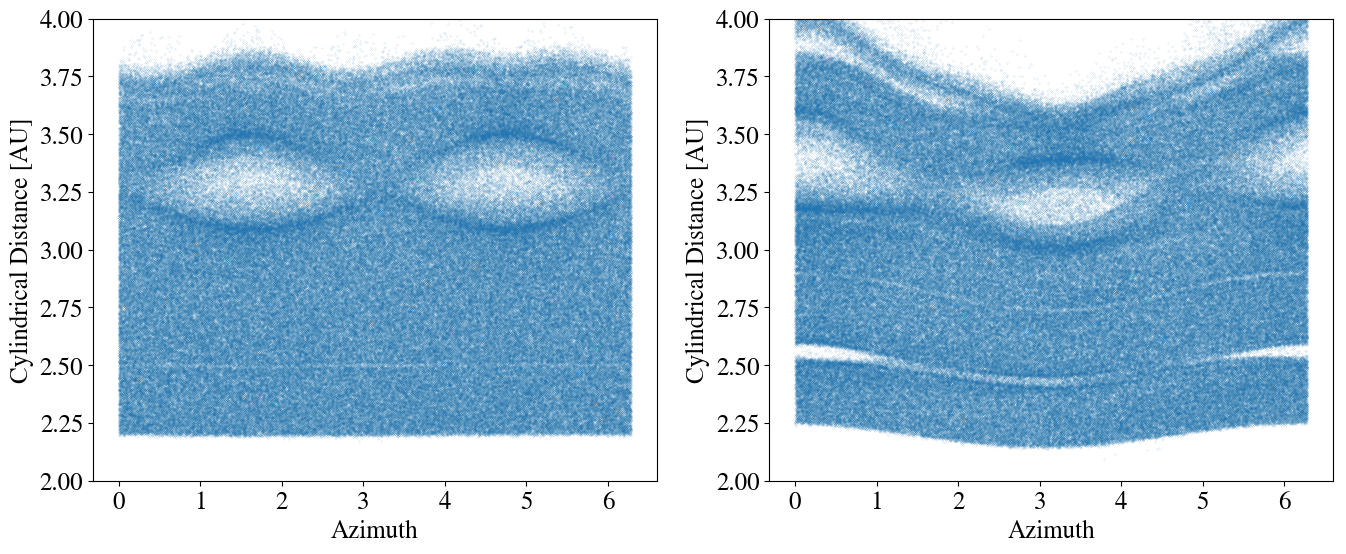
\includegraphics[width=\textwidth]{figures/rtheta.png}
    \caption{Caption goes here.\label{fig:rtheta}}
\end{figure*}

\begin{figure*}
    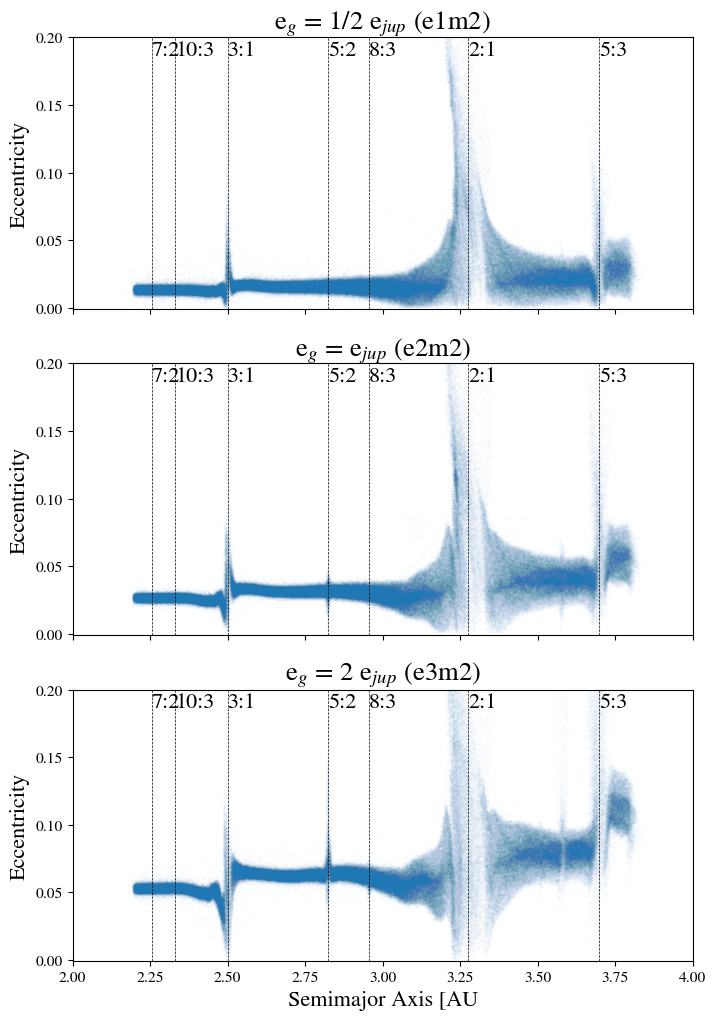
\includegraphics[width=\textwidth]{figures/ae.png}
    \caption{Caption goes here.\label{fig:ae}}
\end{figure*}

\begin{figure}
    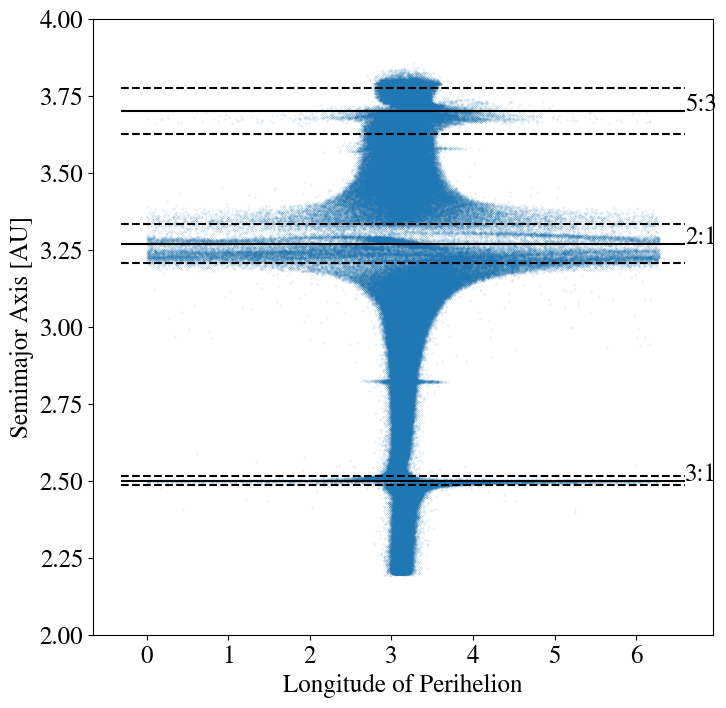
\includegraphics[width=\columnwidth]{figures/long_ph.png}
    \caption{Caption goes here.\label{fig:long_ph}}
\end{figure}

\begin{figure*}
    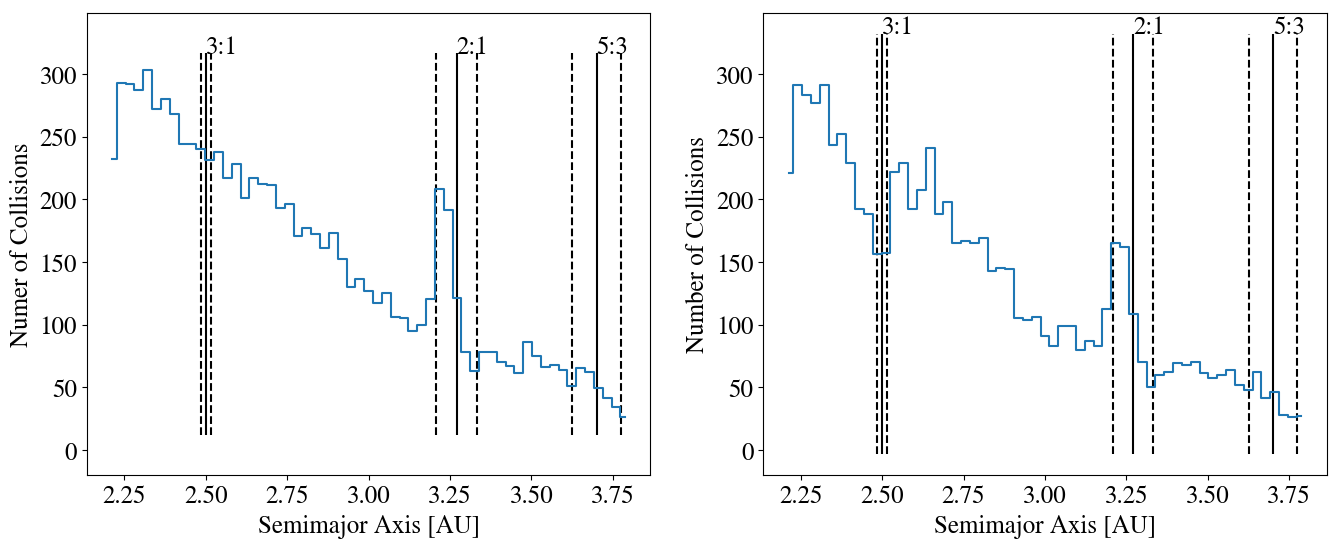
\includegraphics[width=\textwidth]{figures/coll_hist_a.png}
    \caption{Caption goes here.\label{fig:coll_hist_a}}
\end{figure*}

\begin{figure*}
    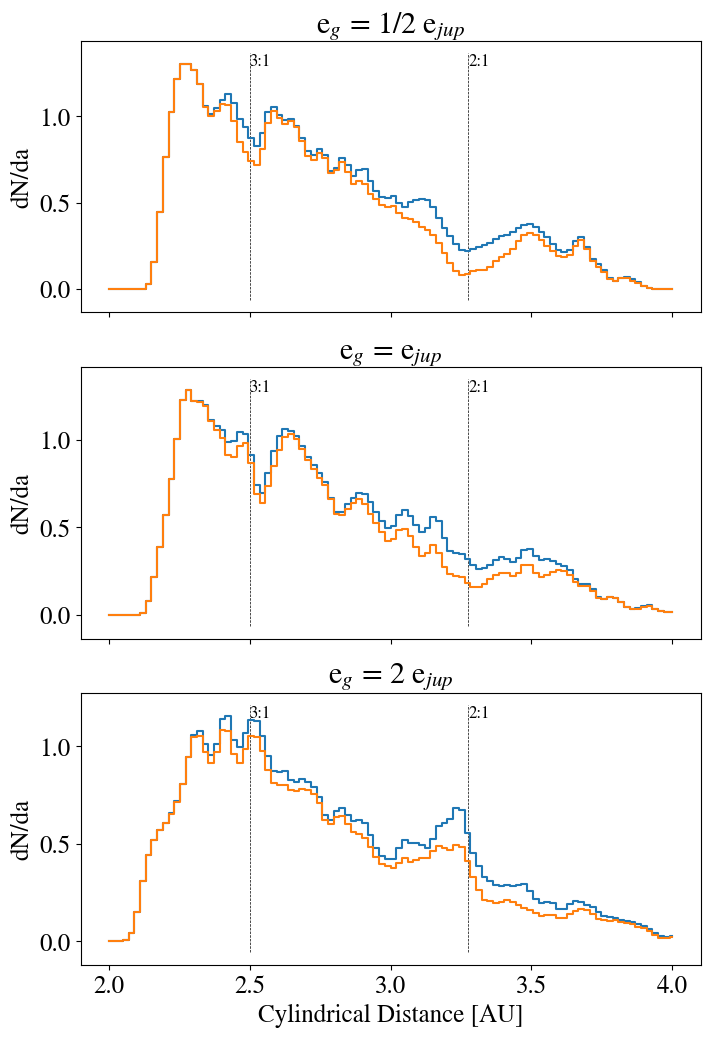
\includegraphics[width=\textwidth]{figures/coll_hist_r.png}
    \caption{Caption goes here.\label{fig:coll_hist_r}}
\end{figure*}

\begin{figure*}
    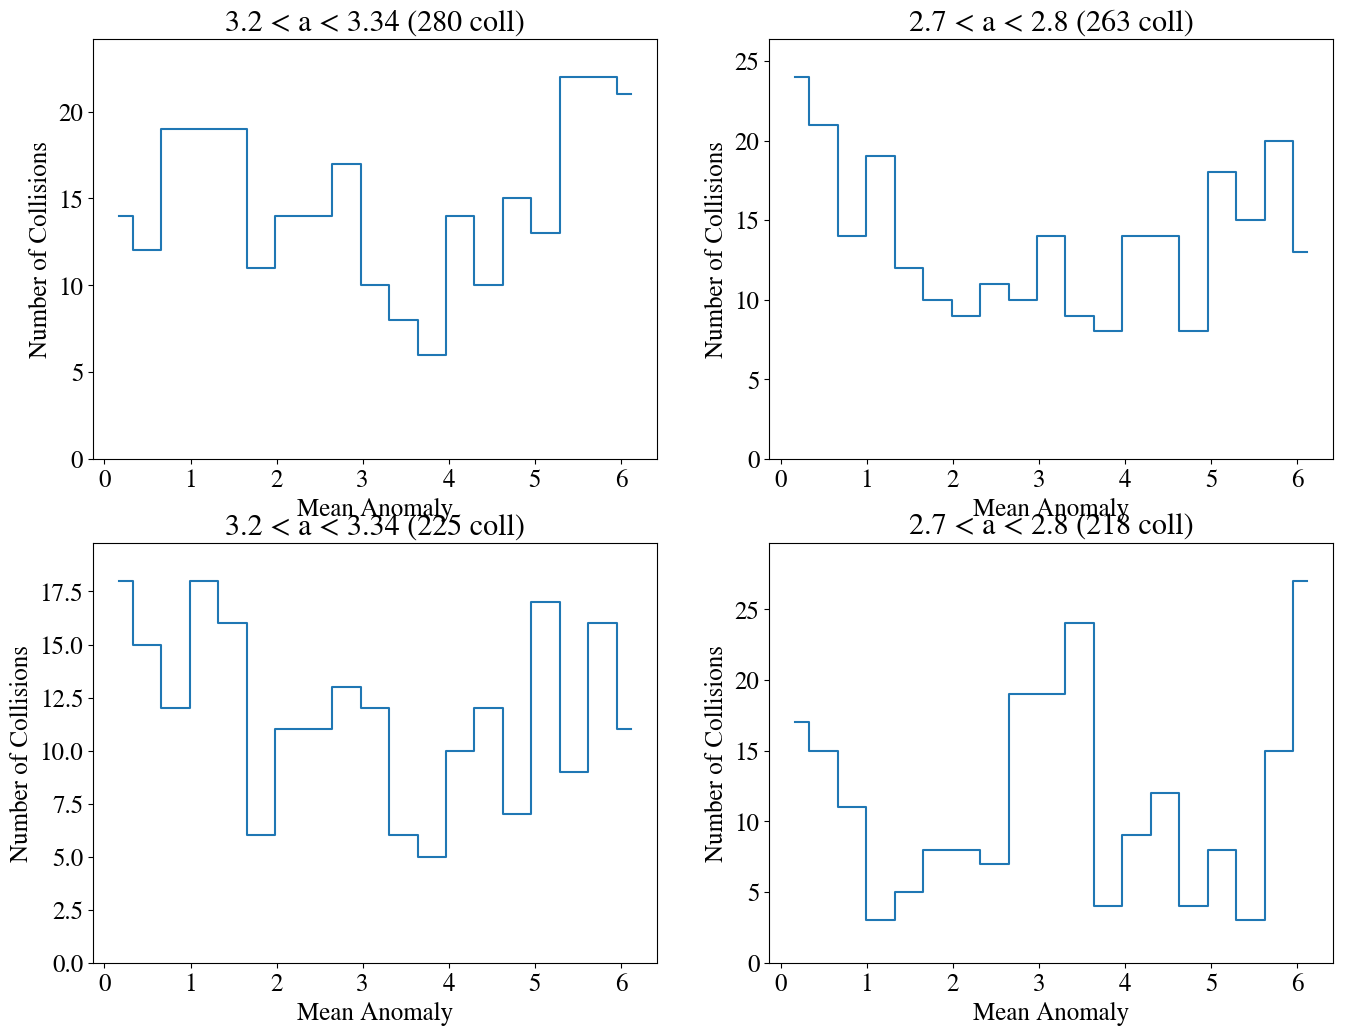
\includegraphics[width=\textwidth]{figures/m_hist.png}
    \caption{Caption goes here.\label{fig:m_hist}}
\end{figure*}

\section{Results} \label{sec:results}

A side-by-side comparison of the final distribution in cylindrical coordinates of planetesimals from the CJ and EJ simulations is shown in figure \ref{fig:rtheta}. Gaps produced by the 3:1, 2:1 and 5:3 MMR with Jupiter are visible in both frames. In the EJ simulation, a gap in the vicinity of the 5:2 MMR is also visible. The non-axisymmetric character of the gaps reflects the fact that the planetesimals in the vicinity of the resonances (especially the 2:1) are having their eccentricities significantly pumped. (I don't think there should be any azimuthal structure to the gaps in the CJ simulation. This is probably a reflection of the fact that we need to run with smaller timesteps.) Although examining the spatial distribution of planetesimals near MMR in debris disks may be a viable way to detect unseen planets, we will not focus on this topic any longer as it has already been covered in detail in other studies \citep{2016ApJ...818..159T, 2018ApJ...857....3T}. It is worth noting, however that the spatial distribution of planetesimals shown in figure \ref{fig:rtheta} appears qualitatively similar to figures 3 and 4 in \citep{2016ApJ...818..159T}.

The location of the mean motion resonances with Jupiter is most clearly visible when examining the semimajor axis-eccentricity distribution of the planetesimals. This is shown in figure \ref{fig:ae}, with the final snapshot from the CJ simulation shown on the left and EJ on the right. The solid vertical lines indicate the nominal locations of the mean motion resonances. Away from the resonance locations, the eccentricity dispersion grows via viscous stirring as energy from the Keplerian shearing of the disk is gradually transferred to random motions of planetesimals. The slight inward curving of the eccentricity peaks near the resonances is a consequence of the conservation of the Jacobi energy. As the semimajor axis of a planetesimal in MMR librates, the corresponding change in eccentricity is given by equation \ref{eq:tiss}.

In the EJ simulation, the eccentricity remains enhanced between the MMRs due to the secular forcing effect of Jupiter. This also has the consequence of making the eccentricity spikes due to the 5:2 and (what's the MMR at 3.6 AU?) more prominent. The reason for this is that the libration width of a resonance generally scales with the eccentricity of the particle being perturbed. In a secularly forced disk, the eccentricity of particles affected by resonance is larger, which increases the resonance width and allows a larger region of the disk to be affected by a given resonance. Also visible in the EJ snapshot in figure \ref{fig:ae} are eccentricity spikes that extend below the background eccentricity distribution. This is a clear sign that planetesimals in the MMRs are librating. The phase of the libration is set by the resonant argument (maybe I should add an equation for the resonant argument in section 2).

An additional effect that the MMRs have on the orbits of planetesimals is visible in figure \ref{fig:long_ph}. This shows the semimajor axis distribution of planetesimals as a function of longitude of perihelion in the EJ simulation. As discussed in section \ref{sec:sec_force}, the eccentric orbit of Jupiter causes the perihelia of the planetesimal orbits to align with the giant perturber. The mean motion resonances, however, drive the rather vigorous precession of the orbits of planetesimals in their vicinity. Because the timescale of the resonances is much shorter than the timescale for secular forcing, the longitudinal orientations of orbits close to the MMRs are effectively randomized. The dashed horizontal lines in figure \ref{fig:long_ph} indicate the libration width of the MMRs at the forced eccentricity (given by the magnitude of equation \ref{eq:eforced}. The size of the zone of vigorous precession roughly matches the libration width of the MMRs. As will be discussed shortly, the relative longitudinal orientation of the orbits has important implications for where and when planetesimal collisions occur at a given semimajor axis. Not shown is the longitude of perihelia and semimajor axes of the bodies in the CJ simulation. Due to the lack of secular forcing, the orientations of the orbits of these bodes are effectively random.

Next, we move on to examine the statistics of the collisions that occur. Figure \ref{fig:coll_hist_a} shows the distribution of semimajor axes of every collision that is resolved. Here, the semimajor axis of a collision is defined as the semimajor axis of the first body participating in the collision at the moment that it occurs. During a collision, the determination of which body is first and which is second is determined by the collision search tree in {\sc ChaNGa}. To ensure that this does not introduce any bias, we also constructed figure \ref{fig:coll_hist_a} using the orbital parameters of the second body and found no qualitative difference. By examining the semimajor axis distribution of the collisions, it is easy to see how the MMRs affect the collision rates. The dashed lines again represent the libration width of each resonance and are meant to show its range of influence. In both the circular and eccentric Jupiter simulations, the collision rate is clearly enhanced interior to the 2:1 MMR. Interestingly, the 3:1 MMR only appears to have a noticemable influence on the collision rate in the EJ simulation. (Better check if this is still true when I rerun CJ with smaller steps). In both cases, the 5:3 MMR appears to slightly enhance the collision rate interior to the nominal resonance location. It is important to keep in mind, however that the libration width of sufficiently eccentric particles near the 5:3 MMR may extend beyond the outer edge of the disk and introduce nonphysical boundary effects.

Although the semimajor axis of a particle at the moment of collision provides useful information about how the mean motion resonances affect the collision rate in the disk, this information alone is not enough to predict where the second generation dust that is produced will end up. To do so, we will operate under the assumption that dust grains produced by collision events will quickly couple to the gas and attain a circular orbit. This assumption, which will be further justified in section \ref{sec:dust}, allows to map the radial variation in the dust surface density to the radial position of the collisions. This is shown in figure \ref{fig:coll_hist_r}, where the histograms indicate the x and y coordinates of a body at the moment that it undergoes a collision. Most notably, many of the prominent features visible in figure \ref{fig:coll_hist_a} no longer appear. This is due to the fact that the orbits of colliding bodies have a wide range of eccentricities. In the CJ simulation, there are prominent dips in the collision rate centered around the 2:1 and 3:1 MMR. Although still visible in the EJ simulation, these dips are much wider and shallower. This is due to the fact that particles near the edge of the region of influence of the MMRs have a higher eccentricity in the secularly forced disk. Because a larger eccentricity allows collisions to happen over a broader range of radial distances, the sharp, well-defined edges of the trough centered around the resonances becomes washed out.

As is seen in figure \ref{fig:long_ph}, the relatively fast precession rates induced by the mean motion resonances overpower the secular forcing by Jupiter and randomize the orientation of orbits near the nominal resonance locations. Of course, this difference in longitude of perihelion of bodies inside and outside of resonance is only present in the EJ simulation because the Jupiter imposes zero forced eccentricity on the disk when it has a circular orbit. Figure \ref{fig:m_hist} provides another view of the difference in collision statistics inside and outside and of resonance. This shows the mean anomalies of bodies at the moment that they undergo a collision. The top row corresponds to the EJ simulation and the bottom rom corresponds to the CJ simulation. The left panels correspond to collisions that occur inside of the 2:1 MMR and the right panels are for collisions that occur with a semimajor axis between 2.7 and 2.8 AU, which is meant to well away from the influence of any resonances. The semimajor axis window size in the right hand panel is chosen so that both histograms contain the same total number of collisions.

The qualitative differences between these four panels can be explained in the following way: for $\approx$ 100 km bodies, gravitational focusing plays a significant role in setting the collision rate. In regions of the disk where the rms eccentricity is small (which corresponds to a small velocity dispersion), the collision rate should be enhanced (see equation \ref{eq:safronov}). Inside of resonances, planetesimals undergo large amplitude libration which pumps up the eccentricity dispersion. This effect is visible in figure \ref{fig:ae} for both the EJ and CJ simulation. This implies that the collision rate should be geometric, and not depend on the velocity dispersion near resonances. When this is true, collisions should preferentially occur near perihelion. The reason for this is that in the geometric limit, the collision probability scales with the ratio between the geometric cross section of the two planetesimals and the surface area of a sphere with radius $r$, where $r$ is the distance between the bodies and the central star. This ratio, and therefore the collision probability, is largest when $r$ is minimized (see \citet{2003AJ....125.2692L}). The fact both of the left-hand panels in figure \ref{fig:m_hist} show a distinct lack of collisions near aphelion is consistent with this explanation.

Note that this trend is not present in the right-hand panels of figure \ref{fig:m_hist}. In the case with Jupiter on a circular orbit (bottom right panel), there is a spike in the collision rate both at perihelion and aphelion. The perihelion spike is still due to the geometric argument presented in the previous paragraph. The aphelion spike is due to the effect of gravitational focusing. At aphelion, bodies achieve their minimum speed. This lowers the relative velocity between planetesimals, which according to equation \ref{eq:safronov} should enhance the collision rate. Note that the collision rate does not exhibit much dependence on mean anomaly outside of resonance in the case with Jupiter on an eccentric orbit (top right panel). This is due to the secular forcing by Jupiter, which aligns the longitude of perihelia of adjacent planetesimals. The result of this is that bodies maintain similar relative speeds over the course of an orbit, even though the orbit is eccentric. This lack of variation in the relative speeds makes collisions equally likely at any orbital phase.

\subsection{Comparison With Analytic Safronov Collision Rate}\label{sec:saf}

Outline for this section:
\begin{itemize}
\item Time evolution of disk surface density for circ and ecc
\item Time evolution of sma vs ecc
\item Number of collisions as a function of sma and radial distance
\item Number of collisions as a function of mean anomaly and delta mean anomaly
\item Comparison between safronov rate and actual collision statistics
\end{itemize}

\section{Dust Emission} \label{sec:dust}

\begin{itemize}
\item Show CASA images
\end{itemize}

\section{Summary and Discussion} \label{sec:discuss}

%In this study, we will consider the effects that an external perturber has on the dynamical evolution and collision rates of planetesimals in a circumstellar disk. Planetesimals are too small to reflect much star light and are of too low mass to have any significant amount of thermal inertial. However, the large amounts of dust produced by collisional grinding can be used to infer where planetesimals are interacting \citep{2005Natur.436..363S, 2015ApJ...806...23L}. Although the behavior of the small dust grains can strongly depend on the hydrodynamic behavior of the gas \citep{2015ApJ...813L..14B}, the evolution of the planetesimals (km sized and larger) should be well decoupled from the gas. This means that results of this study should be applicable to both gas rich protoplanetary disks such as HL Tau and TW Hya, along with dusty debris disks such as Fomalhut \citep{2017ApJ...842....8M}.

%The intermediate stages of planet formation are incredibly difficult to observe. Planetesimals, which are the building blocks of planets, are too small to reflect any significant amount of star light and are of too low mass to carry much thermal inertia. However, large volumes of dust produced through collisional grinding of planetesimals can be used to infer where planetesimals are interacting 

%In the Solar System, the formation of Jupiter is thought to have destabilized the orbits of nearby planetesimals and triggered a short and intense period of bombardment. In addition to triggering a cascade of collisional grinding \citep{2012ApJ...750....8T}, the formation of Jupiter is thought to have facilitated the mixing of volatiles in the inner Solar System \citep{2017Icar..297..134R}.

%From an outsider's perspective, the most easily observable property of the Solar System is the infrared emission from small dust grains. Outside the Solar System, infrared excess has also been tied to the presence of dust (citation needed). Recent high resolution images from ALMA have shown that the structure of these dusty disks around other stars can have rather complicated structures.

%Talk about observed gaps in ALMA images of PPDs. Many different explanations for rings and gaps \citep{2019arXiv190103680V}. One possible explanation is resonances with outer companion. \citet{2017ApJ...850..103B} examined this possibility, but used massless test particles to represent the planetesimals. Although this provided some information about how the planetesimals move under the influence of a mean motion resonance, it did not say anything about where the collisions and dust production would occur.

%Talk about specific PPDs where MMRs might be producing some of the structure (HL Tau, TW Hya)

%Talk about dynamics in MMRs. Resonances tend to push particles away from the perturber. Mention study by \citet{2016ApJ...818..159T, 2018ApJ...857....3T}. Massive disk can move resonance locations (see eq 10 or \citet{2015ApJ...805..100T}). Looks like we are getting a spiral wave being launched from the 3:1 MMR (see section 5.6 in \citet{2016ApJ...818..159T}). Study by \citet{2018MNRAS.473.3547R} used collisionless N-body sim to examine production of cavity in debris disk, assume paricles trace mm sized objects which should be observable.

%See \citet{1984prin.conf..513S} for a fantastic discussion of spiral waves in a planetary context.


%Scattering of planetesimals by giant planet does not depend on migration, so we ignore this process \citet{2017Icar..297..134R}.

Figures to include:

\begin{itemize}
    \item a-e evolution of particles
    \item a-e closeup of resonance (do we need to pick more than one?)
    \item azimuthally averaged profile of collision rates
    \item temporal evolution of collision rates inside and outside resonance
\end{itemize}

Need to expain waves in a-e plots. This is from the free eccentricity cycling through phase space.

Might be useful to compare Aaron's estimate of collsion rates from velocity dispersion in 2017 paper to the actual collision rates that we measure. Collision rates tend to be supressed outside of MMRs compared to Safronov rate. Im guessing this has to do with the fact that precession rates are high inside MMRs and so orbits are not aligned and more likely to cross. For a discussion of secular precession rates due to a giant planet, see \citet{2009MNRAS.399.1403M}.

\bibliography{references}

\clearpage

\end{document}